\documentclass[t]{beamer}
\usepackage{mathtools}
\usepackage{tikz}
\usepackage{pgfplots}
\usepackage{ulem}
\usetikzlibrary{arrows,backgrounds,shapes,matrix,positioning,fit}
\newcommand{\argmax}{\operatornamewithlimits{argmax}}
\newcommand{\argmin}{\operatornamewithlimits{argmin}}
\newcommand{\wt}{\operatornamewithlimits{wt}}
\newcommand{\var}{\operatornamewithlimits{var}}
\renewcommand\Re{\operatorname{Re}}
\renewcommand\Im{\operatorname{Im}}

\mode<presentation>
{
  \usetheme{Singapore}
  %\useoutertheme{infolines} % Showing only current section in navigation
  \setbeamertemplate{headline}{}  % Empty headline
  \setbeamertemplate{footline}[frame number]  % Getting rid of footer items except slide number
  \setbeamercovered{invisible}
  \beamertemplatenavigationsymbolsempty % Getting rid of navigation bullets at the bottom
}
\usepackage[english]{babel}
\usepackage[latin1]{inputenc}
\usepackage{times}
\usepackage[T1]{fontenc}

\title[EE 703 DMT]{Comparison of Modulation Schemes}
\author[Saravanan V]
{
  Saravanan Vijayakumaran\\
  \href{mailto:sarva@ee.iitb.ac.in}{sarva@ee.iitb.ac.in}
}
\institute[IIT Bombay]
{
  Department of Electrical Engineering\\
  Indian Institute of Technology Bombay
}
\date{October 15, 2013}

\AtBeginSection[]%
{%
\begin{frame}[plain]%
  \topskip0pt
  \vspace*{\fill}
    \begin{center}%
      \usebeamerfont{section title}\insertsection%
    \end{center}%
  \vspace*{\fill}
\end{frame}%
}

\begin{document}

\begin{frame}
  \titlepage
\end{frame}

%% Frame %%
\begin{frame}{Metrics for Comparing Modulation Schemes}
  \footnotesize
  \begin{figure}
    \centering
      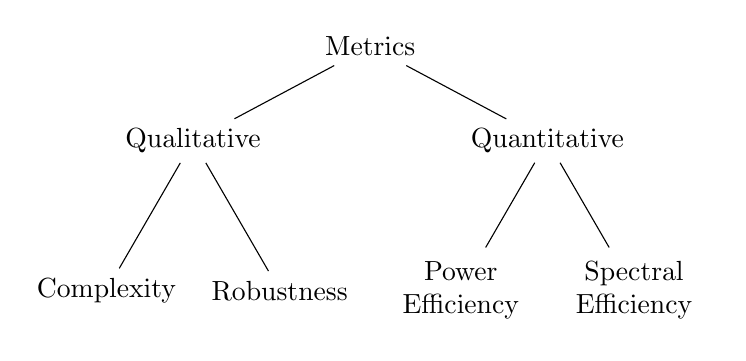
\begin{tikzpicture}[
        level 1/.style={sibling distance=4.5cm,level distance=1.2cm},
        level 2/.style={sibling distance=2.2cm, level distance=1.9cm}
      ]
        \node {Metrics}
          child {
            node {Qualitative} 
            child { node {Complexity} }
            child { node {Robustness} }
          }
          child {
            node {Quantitative}
            child { node {\begin{tabular}{cc} Power \\ Efficiency \end{tabular}} }
            child { node {\begin{tabular}{cc} Spectral \\ Efficiency \end{tabular}} }
          }
          ;
      \end{tikzpicture}
  \end{figure}
  \normalsize
  \end{frame}

%% Frame %%
\begin{frame}{Power Efficiency}
  \footnotesize
  \begin{itemize}
    \item For an $M$-ary signaling scheme
      \begin{eqnarray*}
        P_e & \approx & \pause \bar{N}_{d_{min}} Q\left(\frac{d_{min}}{2\sigma} \right) \\ \pause 
            & = & \bar{N}_{d_{min}} Q\left(\sqrt{\frac{d_{min}^2}{2N_0}}\right) \pause =  \bar{N}_{d_{min}} Q\left(\sqrt{\frac{d_{min}^2}{E_b}}\sqrt{\frac{E_b}{2N_0}}\right) 
      \end{eqnarray*}
    \item \pause The power efficiency of a modulation scheme is defined as
      \begin{eqnarray*}
        \eta_p = \frac{d_{min}^2}{E_b}
      \end{eqnarray*}
    \item \pause The nearest neighbors approximation can be expressed as
      \begin{eqnarray*}
        P_e  \approx \pause \bar{N}_{d_{min}} Q\left(\sqrt{\frac{\eta_p E_b}{2N_0}}\right) 
      \end{eqnarray*}
  \end{itemize}
  \normalsize
\end{frame}

%% Frame %%
\begin{frame}{Power Efficiency of Some Modulation Schemes}
  \footnotesize
  \begin{table}
    \begin{tabular}{ll} 
      Modulation Scheme & $\eta_p$ \\ \hline
      \pause On-off keying & \pause 2 \\
      \pause Orthogonal signaling & \pause 2 \\
      \pause Antipodal signaling & \pause 4 \\
      \pause BPSK & \pause 4 \\
      \pause QPSK & \pause 4 \\
      \pause 16-QAM & \pause 1.6 \\
    \end{tabular}
  \end{table}
  \normalsize
\end{frame}

%% Frame %%
\begin{frame}{Spectral Efficiency}
  \footnotesize
  \begin{definition}[Spectral Efficiency]
    The number of bits that can be transmitted using the modulation scheme per second per Hertz of bandwidth.
  \end{definition}
  \pause
  \begin{block}{Remarks}
    \begin{itemize}
      \item If a modulation scheme transmits $N$ bits every $T$ seconds using $W$ Hertz of bandwidth, the spectral efficiency is $\frac{N}{WT}$ bits/s/Hz
      \item \pause We will use null-to-null bandwidth to calculate spectral efficiency
    \end{itemize}
  \end{block}
  \normalsize
\end{frame}

%% Frame %%
\begin{frame}{Spectral Efficiency of BPSK}
  \footnotesize
  \begin{itemize}
    \item \pause Let $S_p(f)$ be the PSD of BPSK and let $S(f)$ be the PSD of its complex envelope.
      \begin{equation*}
        \pause S_p(f) = \frac{S(f-f_c) + S(-f-f_c)}{2} 
      \end{equation*}
      \pause (Section 2.3.1 of Madhow's book)
    \item \pause The complex envelope is given by
      \begin{equation*}
        s(t) = \sum_{n=-\infty}^{\infty} b_n p(t-nT)
      \end{equation*}
      where $p(t)$ is a rectangular pulse of duration $T$ and $b_n \in \{-A, A\}$. 
    \item \pause Given $S_b(z) = \sum_{k=-\infty}^{\infty} R_b[k]z^{-k}$, PSD of the complex envelope is
      \begin{eqnarray*}
        S(f) = \pause S_b\left(e^{\ j2\pi fT}\right)\frac{\lvert P(f)\rvert^2}{T} = \pause A^2T\text{sinc}^2(fT) 
      \end{eqnarray*}
  \end{itemize}
  \normalsize
\end{frame}

%% Frame %%
\begin{frame}{Power Spectral Density of BPSK}
  \footnotesize
  \begin{figure}
    \centering
      \begin{tikzpicture}[scale=0.5,transform shape]
        \begin{axis}[
                     title={PSD of BPSK Complex Envelope},
                     xmax=7,
                     xmin=-7,
                     ymax=1.5,
                     ymin=-0.5,
                     axis lines = middle,
                     ytick=\empty,
                     xtick = {-5,5,7,-0.5,0.5},
                     xticklabels = {$-f_c$,$f_c$,$f$,$-\frac{1}{T}$,$\frac{1}{T}$},
                     %x tick label style={font=\tiny},
                     x post scale = 2.5
                    ]
          \addplot[color=blue,very thick,domain=-5:5,samples=1000] gnuplot{(sin(pi*2*x)/(pi*2*x))**2};
        \end{axis}
      \end{tikzpicture}
  \end{figure}
  \begin{figure}
    \centering
      \begin{tikzpicture}[scale=0.5,transform shape]
        \begin{axis}[
                     title={PSD of BPSK},
                     xmax=7,
                     xmin=-7,
                     ymax=1.5,
                     ymin=-0.5,
                     axis lines = middle,
                     ytick=\empty,
                     xtick = {-5,5,7},
                     xticklabels = {$-f_c$,$f_c$,$f$},
                     %x tick label style={font=\tiny},
                     x post scale = 2.5
                    ]
          \addplot[color=blue,very thick,domain=-7:7,samples=1000] gnuplot{0.5*(sin(pi*2*(x-5))/(pi*2*(x-5)))**2};
          \addplot[color=blue,very thick,domain=-7:7,samples=1000] gnuplot{0.5*(sin(pi*2*(x+5))/(pi*2*(x+5)))**2};
        \end{axis}
      \end{tikzpicture}
  \end{figure}
  \pause Null-to-null bandwidth of BPSK = \pause $\frac{2}{T}$ (only +ve frequencies)

  \pause Spectral Efficiency of BPSK = \pause 0.5
  \normalsize
\end{frame}

%% Frame %%
\begin{frame}{Spectral Efficiency of Some Modulation Schemes}
  \footnotesize
  \begin{table}
    \begin{tabular}{ll} 
      Modulation Scheme & Spectral Efficiency \\ \hline
      \pause BPSK & \pause 0.5 \\
      \pause BPAM & \pause 1 \\
      \pause QPSK & \pause 1 \\
      \pause 16-QAM & \pause 2 \\
    \end{tabular}
  \end{table}
  \normalsize
\end{frame}

%% Frame %%
\begin{frame}{Spectral Efficiency vs Relative Power Efficiency}
  \footnotesize
  \begin{figure}
    \centering
      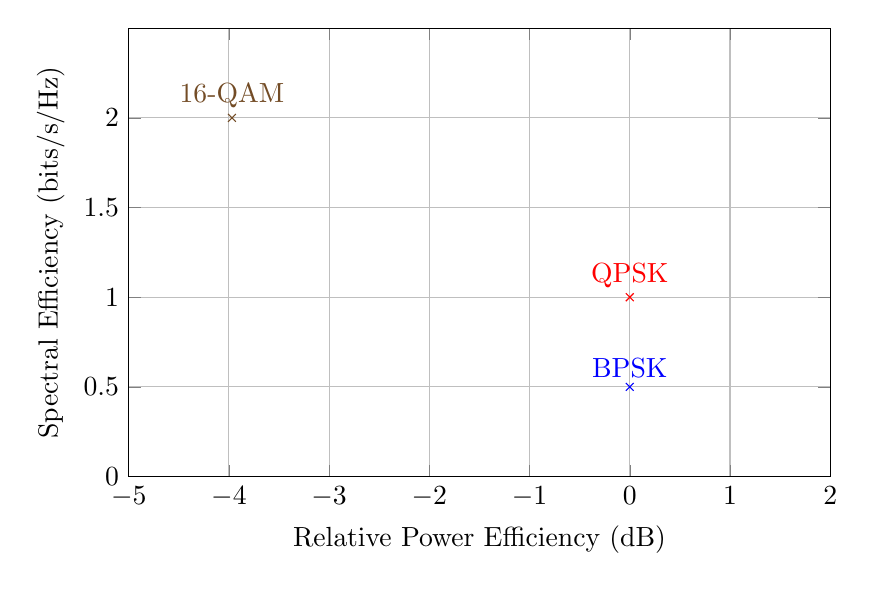
\begin{tikzpicture}[scale=1.0,transform shape]
        \begin{axis}[
            xlabel={Relative Power Efficiency (dB)},
            ylabel={Spectral Efficiency (bits/s/Hz)},
            xmax=2,
            xmin=-5,
            ymax=2.5,
            ymin=0,
            grid=major,
            x post scale = 1.3,
            xtick={-5,-4,-3,-2,-1,0,1,2},
            ytick={0,0.5,1,1.5,2},
            nodes near coords
        ]
          \addplot+[only marks, mark=x, point meta=explicit symbolic] coordinates {(0,0.5)[BPSK]};
          \addplot+[only marks, mark=x, point meta=explicit symbolic] coordinates {(0,1)[QPSK]};
          \addplot+[only marks, mark=x, point meta=explicit symbolic] coordinates {(-3.97,2)[16-QAM]};
        \end{axis}
      \end{tikzpicture}
  \end{figure}
  \begin{eqnarray*}
    \text{Relative Power Efficiency} = 10\log_{10} \frac{\eta_p}{\eta_{p,\text{BPSK}}}
  \end{eqnarray*}
  \normalsize
\end{frame}

%% Frame %%
\begin{frame}{}
\vfill
\begin{center}
Thanks for your attention
\end{center}
\vfill
\end{frame}

\end{document}
